\documentclass[a4paper,14pt]{extarticle}

\usepackage{indentfirst}

\usepackage{xeCJK}
\setCJKmainfont[AutoFakeBold,AutoFakeSlant]{標楷體}
\usepackage{fontspec}
\setmainfont{Times New Roman}

\renewcommand{\baselinestretch}{1.5}
\usepackage{amsmath,amssymb,amsfonts}
\usepackage{algorithm}
\usepackage{algpseudocode}
\usepackage{graphicx}
\usepackage{subcaption}
\usepackage{caption}
\usepackage{xcolor,colortbl}
\usepackage{nicematrix}
\usepackage{cite}
\usepackage{adjustbox}
\usepackage{makecell}
\usepackage{multirow}

\setlength{\parindent}{2em}
\captionsetup[figure]{labelformat={default},name={圖}}
\captionsetup[table]{labelformat={default},name={表}}

\input lstset.tex
\input macros.tex

\algdef{SE}[VARIABLES]{Variables}{EndVariables}
    {\algorithmicvariables}
    {\algorithmicend\ \algorithmicvariables}
\algnewcommand{\algorithmicvariables}{\textbf{initialize variables}}

\renewcommand{\contentsname}{\centering 目錄}

\renewcommand*\footnoterule{}

\makeatletter
\newenvironment{breakablealgorithm}
  {% \begin{breakablealgorithm}
   \begin{center}
     \refstepcounter{algorithm}% New algorithm
     \hrule height.8pt depth0pt \kern2pt% \@fs@pre for \@fs@ruled
     \renewcommand{\caption}[2][\relax]{% Make a new \caption
       {\raggedright\textbf{\ALG@name~\thealgorithm} ##2\par}%
       \ifx\relax##1\relax % #1 is \relax
         \addcontentsline{loa}{algorithm}{\protect\numberline{\thealgorithm}##2}%
       \else % #1 is not \relax
         \addcontentsline{loa}{algorithm}{\protect\numberline{\thealgorithm}##1}%
       \fi
       \kern2pt\hrule\kern2pt
     }
  }{% \end{breakablealgorithm}
     \kern2pt\hrule\relax% \@fs@post for \@fs@ruled
   \end{center}
  }
\makeatother

\urlstyle{same}

\title{應用神經網路架構搜索技術提升YouBike系統之車流預測準確度}

\makeatletter
\newcommand{\printcover}{
    {\fontsize{20pt}{20pt}\selectfont
            \begin{titlepage}
                \begin{center}
                國家科學及技術委員會 111 學年度\\
                \vspace{0.5em}
                大專生計畫結案報告書\\
                \vfill
                \textbf{{\@title}\\
                An Effective Evolutionary Neural Architecture Search for Bike-Sharing System Demand Prediction}\\

                \vfill
                組員:\\
                B084020005 蔡昀燁\\
                B083040012 陳柏翰\\
                B083040022 黃兆延\\
                \vfill
                指導老師:\\
                蔡崇煒\hspace{0.5em}老師\\
                \vfill

                \end{center}
            \end{titlepage}
            \newpage
            \stepcounter{page}
        }
    }
\makeatother

\begin{document}
    \printcover

    \section{摘要}
        近年隨著環保意識和智慧城市的影響,
        公共自行車系統(bike-sharing system ; BSS)因為其環保和便利的特性,
        已然成為各大城市重點發展的公共設施。
        因各站點站位有限,
        可能產生使用者鄰近站點車輛數不足和無站點可停的問題,
        若工作人員無法即時檢修與調度而造成站點的車輛數和空位不平衡,
        將會降低使用者使用意願。
        本專案提出超啟發式演算法(adaptive simulated annealing genetic algorithm ; ASAGA)作為 one-shot 神經網路架構搜尋(neural architecture search ; NAS)的搜尋策略,
        搭配上以混合為基礎的超參數(hyperparameter)優化。
        本專題原計畫利用台灣微笑單車Youbike2.0的資料進行實驗,
        因資料取得較不易以及有缺失的情況,
        我們改用了紐約市公共自行車系統資料,
        建立高效深度學習模型用以預測各站點狀況,
        並期望實際應用於本地高雄市公共自行車系統以解決各站點車輛不平衡之問題。
        期望以預測結果改善現有公共自行車的服務品質,
        提高民眾使用意願,
        最終達到紓困交通且提升營運方收入的效果。
        {\vskip 1em}
        \noindent
        \textbf{關鍵詞}: 神經網路搜索、超參數優化、自行車使用量預測
    \newpage

    \hypersetup{
        breaklinks=false,%
        linkcolor=black,%
        anchorcolor=black,%
        citecolor=black,%
        filecolor=black,%
        menucolor=black,%
        pagecolor=black,%
        urlcolor=black
    }
    \tableofcontents
    \hypersetup{
        breaklinks=true,%
        linkcolor=blue,%
        anchorcolor=blue,%
        citecolor=blue,%
        filecolor=blue,%
        menucolor=blue,%
        pagecolor=blue,%
        urlcolor=blue
    }
    \newpage

    \section{研究動機與研究問題}
        
        公共自行車系統已被許多城市使用多年,
        隨著民眾對自行車系統的認識,
        其便利性、環保等優勢,
        讓使用人數大幅提升。
        使用量的增加產生固定站點的公共自行車系統(dock bike-sharing system)站點車輛數不平衡的問題\cite{chemla2013bike},
        也就是無車可借以及無位可還的狀況,
        此問題影響到使用者的體驗。
        各站點的調度問題牽涉到的因素相當複雜,
        站點自行車數量的變化大致上受到站點周遭人、車流以及使用者習慣兩個重要因素影響;
        站點附近的人、車流會因為站點位置、城市中的大眾交通運輸結構和地理環境而有所不同,
        民眾的使用習慣則會受到當下天氣、道路交通狀況和騎乘用途的影響。
        由於公共自行車有著騎乘路線不固定以及不限於在同一站點租借、歸還的特性,
        公共自行車系統的站點需求預測至今仍是各廠商致力完成的目標,
        許多學者也開始將日漸發展成熟的深度學習技術應用於公共自行車的實務問題上,
        嘗試解決這道複雜的難題。
      
        近年來由於深度學習在電腦視覺領域獲得突破性的發展\cite{8114708},
        將深度學習應用於自行車站點車輛數預測成為本專案的研究重點。
        目前所被大眾熟知的深度學習模型包括VGG16\cite{simonyan2014very}、ResNets\cite{he2016deep}等皆為卷積神經網路(convolutional neural network ; CNN),
        其處理的資料多為圖像,
        然而不同於許多影像辨識的資料集,
        處理公共自行車系統資料時不只需要考慮各站點之間所蘊含的空間特徵,
        其時序性也是重要的參考依據,
        因此空間-時間混合的神經網路模型(spatial - temporal hybrid model)成為現今預測交通流的重要方法之一。
     
        為了讓深度學習模型在其應用的問題上得出最佳的結果,
        必須對模型的架構和參數進行調整,
        包括資料的選擇、超參數的數值(hyperparameter tuning)\cite{10.5555/2986459.2986743}、資料的前處理(data preprocessing)\cite{kotsiantis2006data}\cite{famili1997data}以及神經網路架構的設計。
        進行人為調整需要特定領域的專業背景知識並花費大量時間,
        能夠自動生成高預測準確率模型架構的自動化機器學習(automated machine learning)\cite{WARING2020101822}因而成為近年的熱門主題,
        其中又以神經網路架構搜尋\cite{elsken2019neural}最受矚目。
        然而在大量的超參數需要被考慮進NAS的搜尋空間(search space)時,
        使用NAS建立合適的模型將需要大量的計算資源\cite{zhao2020simplifying}。
        為了解決此問題,
        本專題製作利用one-shot NAS方法\cite{pmlr-v80-bender18a}建立一個超級網路(supernet),
        並提出 ASAGA 作為搜尋策略,
        生成最佳的神經網路架構預測腳踏車系統中各站點的車輛數,
        減少搜索時間與大量的計算資源消耗,
        期望在有限時間、計算資源的情況下獲得高準確度的結果,
        並投入至本地公共自行車系統來解決腳踏車分配不平衡的問題。
    \newpage

    \section{文獻回顧與探討}
        \subsection{交通流預測模型相關研究}
            
            交通流(traffic flow)擁有高度的時序及空間之關聯性質,
            卷積長短期混合模型(CNN-LSTM hybrid model)因而成為眾多研究所使用的預測方法。
            利用卷積神經網路提取空間特徵及長短期記憶模型(long short-term memory ; LSTM)挖掘時間特徵,
            把交通流的時間及空間特性一同進行處理。
            Narmadha等人\cite{NARMADHA2021}建構了多變量的卷積長短期記憶混合模型(multivariate CNN-LSTM),
            藉由混合一維卷積層(CNN layers)及長短期記憶的框架來預測多變量的輸入,
            並與其他五種監督式學習方法比較,
            實驗結果顯示混合模型的準確度超越了其他的非混合模型。
            Zheng等人\cite{8171119}則是根據交通流所蘊含的周期性,
            推斷不同日期的同個時段可能會有相似的車流與人流變化,
            基於此理論在基礎的卷積長短期記憶混合模型上搭配雙向長短期記憶模型(Bi-directional LSTM),
            得到更為完整的時間性資料,
            並從實驗結果證實一定程度上參照未來的時間段能夠有效提升預測準確率。
            Mihaita等人\cite{8916852}對混合模型提出了疑問並實驗測試,
            將卷積神經網路及長短期記憶模型分離出來,
            發現單獨使用長短期記憶模型比起卷積長短期記憶混合模型更加準確,
            推斷卷積神經網路在某些狀況下反而會拖累整體表現。
    
        \subsection{腳踏車共享系統之站點預測相關研究}
            
            現今的腳踏車共享系統大多具有固定站點的特性,
            在與系統相關的應用問題中,
            經常使用站點的車輛變化作為預測目標,
            例如:調整各站點自行車數量來改善使用者體驗、分析各站點資訊來決定是否需要增設站點\cite{PARK2017154}等。
            Lu\cite{9093851}及Zhou\cite{8621918}等人透過在資料集中加入興趣指數(point of interest ; POI),
            突顯各站點的空間特徵,
            並利用循環神經網路(recurrent neural network ; RNN)進行訓練,
            有效地提高了預測站點車輛變化的準確度。
            Yang等人\cite{YANG2020101521}以圖論為基礎,
            針對各站點新增特徵點,
            例如單一站點在特定時間內的車輛流入量(inflow)等,
            並利用機器學習模型預測紐約市共享自行車的各站點需求量。
         
            不少研究都開始採用深度學習的方式\cite{Lv2015TrafficFP}來進行交通流的預測。
            為了取得用傳統機器學習方法無法發覺的潛藏特徵,
            越來越多的研究將交通資料當作類影像資料並使用卷積神經網路來捕捉其中的空間資訊。
            Shi\cite{shi2015convolutional}等人建立了卷積長短期記憶模型(convolutional long short-term memory)來處理空間與時間的相互依賴性(spatio-temporal dependency),
            在降雨預測上獲得不錯的實驗成果,
            證明了時間與空間的關聯性(spatio-temporal correlation)對於預測連續時序性的目標是非常關鍵的。
            Yao等人\cite{yao2019revisiting}提出了空間-時間混合的動態深度學習框架(spatial-temporal dynamic network ; STDN)來進行交通流預測,
            不像是先前的研究將空間與時間的相互依賴性離散化地處理,
            STDN藉由同時考慮每個站點之間的空間資訊與時間連續關係,
            妥善地處理交通流資料空間與時間的相互依賴性,
            實驗結果表明了STDN比起其他方法有更高的準確率。

        \subsection{神經網路架構搜尋相關研究}
            
            神經網路架構搜尋的目的為利用一套演算法或是框架自動根據需求找出最好的神經網路架構,
            最早的神經網路架構搜尋由Zoph等人\cite{zoph2016neural}所提出,
            基於強化學習(reinforcement learning),
            利用控制器(controller)從搜尋空間中找出一個神經網路架構進行訓練,
            並根據評價(evaluate)結果所獲得的獎勵(reward)來更新控制器,
            讓控制器學習如何從搜尋空間中找出更好的神經網路架構。
            但在沒有限制搜尋空間的情況下,
            利用強化學習作為搜尋策略需要反覆多次訓練模型,
            造成搜尋成本相當龐大,
            如果沒有足夠的運算資源會非常耗費時間,
            無法應用在真實世界的問題上。
            Wang等人\cite{8477735}有鑑於神經網路架構搜尋花費時間過長,
            改良並採用粒子群最佳化(particle swarm optimization ; PSO)來優化整體框架。
            藉由引入網路協定地址(internet protocol address ; IP address)的編碼方式及殘缺層(disabled layer),
            解決傳統粒子群演算法無法應用於可變層數(variable-length)的問題,
            實驗結果也證明可變層數的神經網路架構搜尋在準確率上有顯著提升。
            Sun等人\cite{8712430}提出了演化式卷積神經網路(evolutionary convolutional neural network ; EvoCNN),
            以基因演算法(genetic algorithm ; GA)為基礎,
            使用標準差(standard derivation)及平均值(mean value)為代表性資料,
            減少所需的運算資源與時間,
            結果表明演化式卷積神經網路能夠以更少的參數(parameters)在更短的的訓練週期(epoch)得到更好的結果。

        \subsection{One-Shot NAS及搜尋策略相關研究}
            
            Brock等人\cite{brock2017smash}訓練一個超級網路來生成不同模型架構的權重,
            利用超級網路和常規訓練兩者分別所得權重之模型在預測結果上的高度相關性,
            驗證大量的神經網路架構並依照性能進行排序,
            更有效率地篩選出性能較佳的模型架構。
            首先建立一包含所有候選模型架構(candidate architecture)的超級網路,
            在每一次的訓練過程中隨機取樣一網路架構並利用超級網路生成該架構的權重,
            接著再利用所得誤差對超級網路進行反向訓練。
            超級網路訓練完畢後,
            從中隨機取樣架構並使用先前所得權重驗證其性能,
            藉以篩選出性能較佳的模型,
            這樣的方法透過訓練一次超級網路而非重複訓練不同架構來減少搜尋的時間。
            根據不同訓練超級網路的方法,
            許多one-shot NAS框架的變體也相繼被提出。
            高效率神經網路架構搜尋(efficient neural architecture search ; ENAS)使用近似梯度(approximate gradients)\cite{pedregosa2016hyperparameter}來進行強化學習,
            模擬結果顯示ENAS在CIFAR-10資料集只有2.89\%的錯誤率。
            可微分式神經網路架構搜尋(differentiable architecture search ; DARTS)\cite{liu2018darts}以梯度優化為主軸,
            實驗結果顯示DARTS在影像分類及語言模型化的任務準確率上超過了當代不使用微分策略架構搜尋之框架,
            並且有更好的搜尋效率。
            
            單路徑~one-shot~神經網路架構搜尋~(single path one-shot neural network architecture search : SPOS)~\cite{guo2020single}
            在訓練階段採用均勻抽樣~(uniform sampling)~來讓所有子架構獲得平等的訓練,
            並使用演化式演算法~(evolutionary algorithm)~評估架構,
            結果顯示~SPOS~在ImageNet資料集上可以有效的提升準確率。
            在神經網路架構搜尋的框架中,
            搜尋策略對於搜尋的成果和時間成本有著決定性的影響,
            許多研究開始使用演化式演算法來加速模型的評量\cite{6791438};
            Real\cite{real2019regularized}的研究顯示相對於隨機搜尋和強化式學習,
            使用演化式演算法來搜尋架構可以取得更好的效率及準確率。

        \subsection{自動化機器學習相關研究}
            當今的機器學習在各方面的表現都相當出色,
            其中類神經網路尤為突出。
            然而真實世界的大多非常複雜,
            為處理這些困難的問題,
            使用的模型通常都經過精心的設計,
            如前述的神經網路架構搜尋或超參數優化等。
            這對於一般使用者造成了極大的困擾,
            在缺乏資料科學與該問題所屬的專業領域知識下,
            使用者很難找出最適合該問題的最佳配置。
            在這樣的發展背景下,
            自動化機器學習逐漸成為人工智慧領域的一大研究要點。
            Guyon等人\cite{pmlr-v64-guyon_review_2016}主導了一場沒有人為干涉的自動化機器學習挑戰,
            其中的參賽隊伍不乏Intel及AAD Freiburg強力隊伍。
            Intel隊伍提出了一個以樹架構(tree)為基底的C/C++實作,
            在隨機子空間(random subspace)動態調整已學習特徵之間的關聯,
            配合梯度加速(gradient boosting)來快速地建構所使用的樹模型。
            這套軟體最初是用以加速與優化半導體製程,
            也因為其商業性,
            Intel官方並沒有公開相關程式碼。
            AAD Freiburg則是將第三方機器學習庫sckit-learn與連續模型基準型演算法調教(Sequential Model-Based Algorithm Configuration ; SMAC)結合,
            嘗試挖掘出目前資料集最適合的管線(pipeline),
            並在最後將組合篩選(ensemble selection)將這些輸出合併在一起。
            在這個競賽中可以見得組合學習(ensemble learning)在自動化機器學習方面有極高的潛力,
            但究竟是同質性(homogeneous)組合還是異質性(hetrogeneous)組合較為有效至今能未有個定論。

            演化式計算常被用來在時間與資源壓力下找出近似最佳解。
            Real等人\cite{pmlr-v119-real20a}提出了AutoML-Zero這個框架,
            導入了簡單的基因演算法概念,
            將機器學習程式碼以更簡易的數學符號抽象化,
            打破了自動化機器學習長久以來需人為事先規定好搜尋空間的做法,
            進而發掘人為設計時可能遺漏的優秀方法。
            在減少了人為干擾後,
            搜尋空間會稀疏許多,
            即使是簡單的線性回歸問題都可能難以找到適合的參數,
            為此加入了代理任務(proxy task)與遷徙(migration)機制,
            提升AutoML-Zero搜尋的速度。
            實驗結果表明此做法能有效演化出高準確率的神經網路模型,
            即使只有使用簡單的數學符號為基本單位,
            AutoML-Zero依然能自己拼湊出當今常用的機器學習與神經網路優化技術,
            如:干擾資料(noise data)、相乘互動性(multiplicative interactions)、感知平均(average perceptron)、權重平均(weight average)、正規化等等,
            側面證明了其效力。
            Liang等人\cite{10.1145/3321707.3321721}認為自動化機器學習不只要能搜尋到好的架構,
            同時模型超參數的調校也是必不可缺的。
            他們提出了演化式學習人工智慧框架(learning evolutionary AI framework ; LEAF)來完成這2個目的。
            LEAF由3個部分組成:演算法層、系統層與問題-領域(problem-domain)層。
            演算法層的核心為共同演化深度變化結構神經進化(coevolution deep neuroevolution of augmenting topologies ; CoDeepNEAT),
            常被用函式優化(function optimization)、子程序優化(subroutine optimization)及捕食者-獵物動力學(predator-prey dynamics)。
            系統層是演算法層與雲端運算的應用程式介面(application programming interface ; API),
            當個體訓練完成時將所需資訊記錄下來。
            問題-領域層最重要的工作就是優化超參數、架構搜尋與縮小複雜度,
            這也是該框架最核心的部分。
            考量到計算所需的硬體設備與時間,
            LEAF採用了帕雷托排序(Pareto Front)的方式計算適應度,
            結果表明這樣的評價方式能有效地在準確率與模型大小之間取得一定程度的平衡。
        
        \subsection{重要參考文獻之評述}
            本專案擬開發新型共享單車管理系統,
            討論近期新興技術,
            其中含括了交通流與自行車系統站點預測、深度學習改良技術(神經網路架構搜尋、神經網路超參數最佳化、自動化機器學習)和超啟發式演算法(基因演算法與模擬退火演算法)。
            \xtab{tab:related_work}進一步整理這些研究之中較為重要的相關研究,
            並說明這些方法的基本概念。
            本計畫預計發展一個以神經網路架構搜尋及超啟發演算法來提升以深度學習方法為基礎之共享單車系統效能,
            下列將分別介紹【神經網路架構搜尋】及【超啟發式演算法】相關重要參考文獻之評述。
            STDN\cite{yao2019revisiting}在腳踏車與計程車車流部分都有優異的預測結果,
            但資料集為預先收集好的歷史站點資料,
            模型設計與參數可能不適用於變化頻繁的即時性資料,
            這也是我們在專案中導入神經網路架構搜尋和超參數優化的主因。
            NAS\cite{zoph2016neural}與LEAF\cite{10.1145/3321707.3321721}雖然能從龐大的搜尋空間中找出可行的模型架構,
            消耗掉的計算資源與時間也同樣非常可觀,
            SMASH\cite{brock2017smash}嘗試運用超級網路與共同權重訓練策略來減少傳統神經網路架構搜尋的龐大計算量,
            成功發展出一套可行的神經網路架構搜尋框架。
            現今大多數自動化機器學習都採用了超啟發式演算法,
            演化式計算是最典型的例子,
            然而基因演算法容易過早收斂陷入區域最佳解,
            若能發展一個更為優異的解空間資訊引導用的超啟發演算法應用於神經網路架構搜尋,
            將能此領域帶來劃時代的變革。
            從深度學習(監督式學習)、超啟發式演算法(非監督式學習)及智慧單車共享系統,
            我們歸納出幾個與本研究計畫相關的重點研究議題:
            \begin{itemize}
                \item
                神經網路架構搜尋技術實際應用於單車共享系統預測時應考慮考慮架構大小、記憶體需求、計算速度與計算速度。
                \item
                神經網路架構搜尋與超參數優化的解空間非常廣大且稀疏,
                需要一個高效率的超啟發演算法來快速找到可行解。
                \item
                美觀且方便的操作介面能讓一般用戶及管理人員在使用系統時能大幅提升操作體驗,
                加強本系統的未來發展性。
            \end{itemize}
            考量上述研究議題,
            本計畫將嘗試發展一個混合式的【高效超啟發式演算法】,
            進一步發展一個【準確的神經網路架構搜尋框架】,
            應用於共享單車系統達到透過人工智慧驅動交通建設發展的目標。
            \begin{table}[htbp]
                \begin{NiceTabular}{|m[c]{8em}|m[c]{7em}|m[c]{18em}|c|}
                    \CodeBefore
                        \rowcolor[HTML]{C0C0C0}{1}
                        \rowlistcolors{2}{white, gray!25}[restart]
                    \Body
                        \hline
                        方法 & 方法簡稱 & 方法簡介 & 時間 \\
                        \hline
                        \Block{2-1}{交通流預測模型} & multivariate CNN-LSTM\cite{NARMADHA2021} & 混合多層一維卷積層(CNN layers)及長短期記憶網路的混合模型來,獲得比起傳統時序模型更加準確的預測結果。 & \\
                        & Bi-directional LSTM\cite{8171119} & 使用雙向的長短期神經網路攫取更多車流資料中的時域相似度,解決單方向長短期神經模型容易忽略時間相關性之問題。 & \\
                        \hline
                        \Block{2-1}{腳踏車共享系統之站點預測} & POI\cite{9093851}\cite{8621918} & 利用興趣指度強調站點附近特徵,提高空間資訊在預測模型中的效果。 & \\
                        & STDN\cite{yao2019revisiting} & 同時考量每個站點之間的空間資訊與時間連續關係,加上注意力與車流閥門機制來預測各站點自行車使用情況。 & \\
                        \hline
                        \Block{2-1}{神經網路架構搜尋} & NAS\cite{zoph2016neural} & 用強化學習與獎勵機制訓練控制器,並根據回饋來更新控制器,從搜尋空間中找出適用的神經網路架構。 & \\
                        & EvoCNN\cite{8712430} & 以標準差及平均值為代表性資料,利用演化式搜尋減少所需的運算資源與時間。 & \\
                        \Block{2-1}{One-Shot NAS及搜尋策略} & SMASH\cite{brock2017smash} & 利用超級網路和常規訓練兩者分別所得權重之模型在預測結果上的高度相關性,高效率地找出優秀的神經網路架構。 & \\
                        & SPOS\cite{guo2020single} & 採用均勻抽樣讓所有子架構獲得平等的訓練,搭配演化式計算評估架構,減少訓練所需的時間。 & \\
                        \Block{2-1}{自動化機器學習} & AutoML-Zero\cite{pmlr-v119-real20a} & 將機器學習程式碼以簡易的數學符號抽象化,加上代理任務與遷徙機制,能有效演化出高準確率的神經網路模型。 & \\
                        & LEAF\cite{10.1145/3321707.3321721} & 共同演化深度變化結構神經進化配合帕雷托排序的多目標設計,能夠自動找出所需的神經網路模型。 & \\
                    \end{NiceTabular}
                \label{tab:related_work}
            \end{table}
        
    \newpage

    \section{研究方法}

        \begin{table}[tbh]
        \setlength{\belowcaptionskip}{12pt}
        \caption{
            {\fontsize{12pt}{10pt}\selectfont
                \textbf{符號表}
            }
        }
        \centering
        \begin{NiceTabular}{|l|l|}
            \CodeBefore
                \rowcolor[HTML]{C0C0C0}{1}
                \rowlistcolors{2}{white, gray!25}[restart]
            \Body
                \hline
                \textbf{符號} & \multicolumn{1}{c}{\textbf{定義}} \\
                \hline
                $a$ & 興趣點地圖的種類(在此研究中有10種分類) \\ 
                \hline
                $i$ & 站點$i$ \\
                \hline
                $x$ & 興趣點地圖的座標 \\
                \hline
                $M_{i,x}^{a}$ & 在種類$a$、站點$i$、座標$x$網格中的興趣指數 \\
                \hline
                $\mu_{i,x}^{a}$ & 在種類$a$、站點$i$、座標$x$網格中的評價總數 \\
                \hline
                $\gamma$ & 在種類$a$、站點$i$、座標$x$網格中興趣地點的數量 \\
                \hline
                $\rho$ & 在單個網格中的平均評價 \\ 
                \hline
            \end{NiceTabular}
            \label{tab:notation}
        \end{table}

        \begin{figure}[h]
            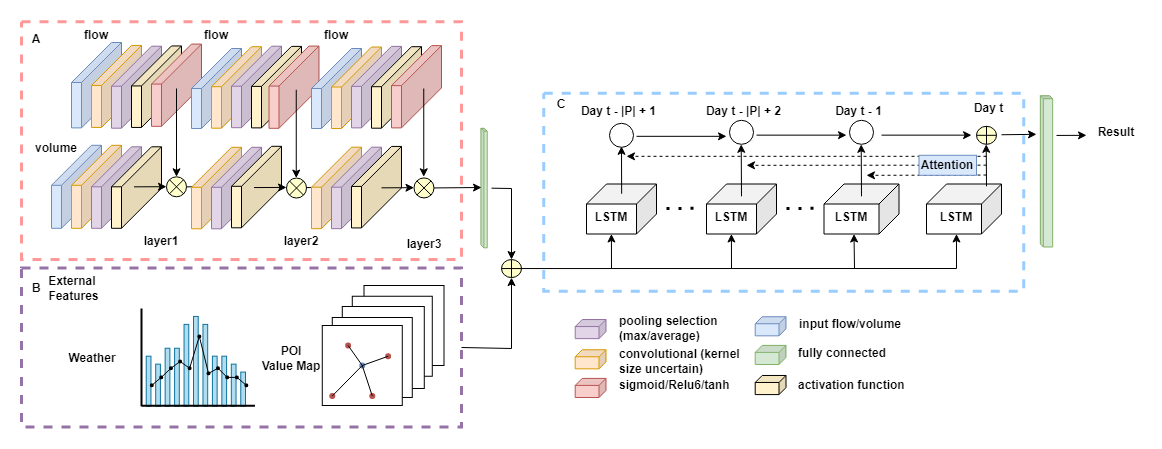
\includegraphics[width=\textwidth]{SAGAON.png}
            \caption{
                {\fontsize{12pt}{10pt}\selectfont
                    SAGAON的架構。
                    (A) 站點車輛數目跟車流量資料會經過數層卷積層。
                    one-shot NAS會同時訓練多個包含不同卷積核大小、池化層和激勵函數的選擇模塊。
                    (B) 採用天氣和興趣指數等額外特徵,
                    該模型可以學習更多影響到公共自行車系統行為模式的外部因素。
                    (C) 使用長短期記憶模型來捕捉腳踏車車流的週期性。
                    $P$代表長短期記憶模型所考慮的天數,
                    而$t$則是代表預測目標的時段(timeslot)。
                }
            }
            \label{fig:SAGAON}
        \end{figure}

        為了能讓模型更好地理解交通流資料中空間與時間的相互依賴性以及利用神經網路架構搜尋建立更好的架構,
        我們提出了一個全新的神經網路架構搜尋框架-模擬退火基因演算法one-shot神經網路搜尋(simulated annealing-genetic algorithm one-shot network ; SAGAON)。
        \xfig{fig:SAGAON}為SAGAON框架的示意圖,
        主要分為3個部分。
        首先\xfig{fig:SAGAON}(A)中的複數卷積層捕捉空間特徵,
        其結果會與\xfig{fig:SAGAON}(B)的額外特徵進行串接。
        在得到空間特徵之後,
        資料將會被送到\xfig{fig:SAGAON}(C)部分的長短期記憶模型來解析時序特徵。
        最後SAGAON將會得到一個超級網路並使用ASAGA演算法來搜尋與公共自行車需求問題相對應的最好架構。
        
        \subsection{空間與時間的相互依賴性}
            \label{subsec:spatial_temporal}
            
            Li等人\cite{li2015traffic}根據地理位置將站點分群,
            並以群為單位進行預測,
            藉此減少模型的複雜度,
            不過考慮到公共自行車系統的真實使用情境,
            我們選擇預測單一站點的車流,
            並利用分群結果計算車流量(flow)特徵來增強每個站點對彼此流量關係的理解。
            我們使用3層的卷積層來讀取空間特徵,
            並以每個站點的站點車輛數目(volume)以及車流量為輸入。
            在每一層中,
            這兩種輸入都會經過3個線性選擇模塊(linear choice block),
            分別是 (1) 卷積核大小(kernel size) (2) 最大或平均池化層(max/average pooling) (3) 激勵函數(activation function),
            在時段$t$第$i$站點的卷積層結果表示成$R_{i,t}$。
            \xfig{fig:SAGAON}(C)部分採用跟STDN相似的結構,
            由複數的長短期記憶層(LSTM layer)組成,
            為了將不同時間尺度的腳踏車車流週期性納入考量,
            每個長短期記憶層都會接收\xfig{fig:SAGAON}(A)前幾個時間段的輸出並加上\xfig{fig:SAGAON}(B)的額外特徵(天氣和興趣指數)來獲取空間及時間特徵。
            在這裡我們使用注意力機制(attention mechanism)來評斷每個時間段對時序預測的影響,
            用以捕捉近期車流週期性的細微差異。
            我們使用的長短期記憶模型是Hochreiter\cite{10.1162/neco.1997.9.8.1735}所提出的原始版本,
            $R_{i,t}$和$e_{i,t}$分別為站點$i$在時間段$t$的卷積結果與額外特徵,
            $h_{i,t}$則代表長短期記憶模型的輸出結果。
            長短期記憶模型的公式如下:
            \begin{equation}
                h_{i,t} = \text{LSTM}([R_{i,t};e_{i,t}],h_{i,t-1}).
            \end{equation}

        \subsection{One-Shot NAS 及自適應退火基因演算法}
            
            \begin{figure}[htb]
                \centering
                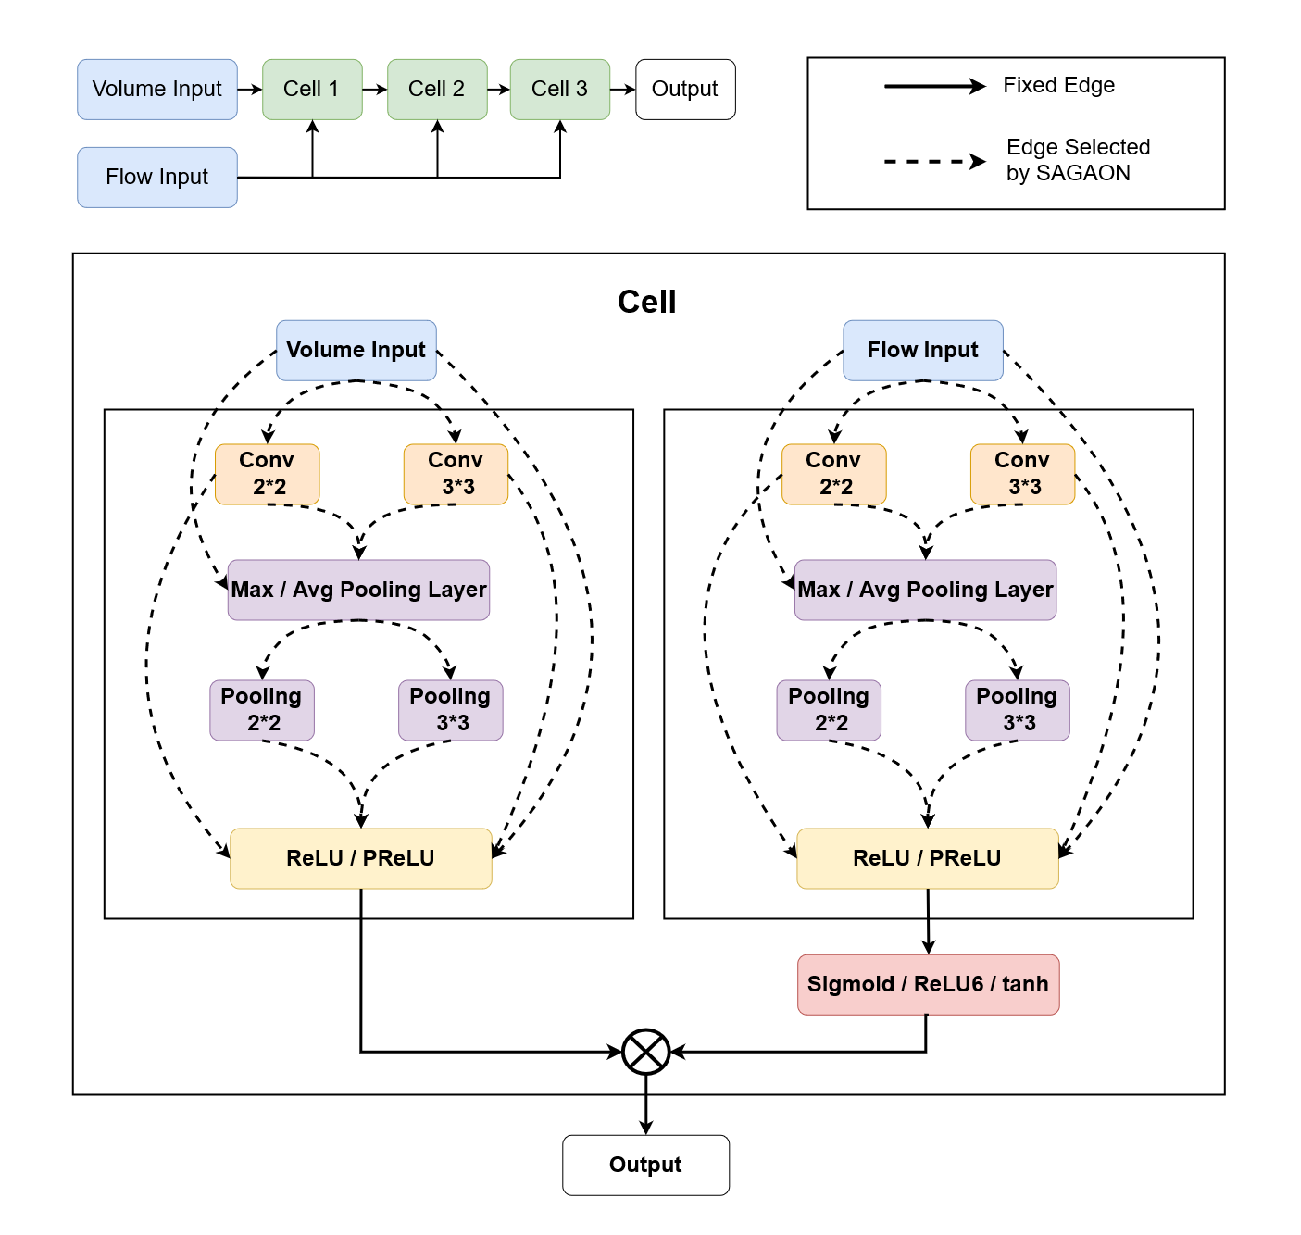
\includegraphics[width=0.8\textwidth]{cell.pdf}
                \caption{
                    {\fontsize{12pt}{10pt}\selectfont
                        元件與選擇模塊。
                        站點車輛數特徵以及車流量特徵會經過三層元件,並在選擇模塊中隨機選擇不同的
                        卷積核大小、池化層以及激勵函數。
                        圖中的實線為固有的模型架構,虛線為經過隨機選擇的可能結果。
                    }
                }
                \label{fig:cell}
            \end{figure}

            為了減少搜尋架構的時間,
            Guo\cite{guo2020single}提出了採用均勻抽樣的單路徑one-shot神經網路架構搜尋。
            透過這個方法能夠減少搜尋時間,
            同時維持搜尋成果的準確率。
            \xfig{fig:cell}展示了元件(cell component)的內部狀況,
            基於STDN的原有架構,
            我們在每個超級網路的元件裡面建立了3個選擇模塊,
            將不同的卷積核大小(kernel size)和激勵函數(activation function)加入SAGAON的搜尋空間,
            並新增池化層(pooling layer)擴充原有的架構,
            除了上述的選擇外,移除特定的架構也是搜尋空間中的一種選擇,藉此增加可搜尋的模型架構數量。
            在SAGAON裡,
            三種不同層級的元件被設置在處理空間特徵的\xfig{fig:SAGAON}(A)部分。
            為了避免不同大小的矩陣發生無法進行計算的情況,
            經過卷積和池化後將會使用零填充(zero padding)維持矩陣大小的一致性,
            保證接下來的矩陣乘法可以順利運行。
            車流量輸入的部分,
            在進行矩陣乘法之前會先經過S型函數(sigmoid function),
            避免車流量的特徵值成長過於迅速。
            在產生超級網路之後,
            我們使用了結合基因演算法和模擬退火演算法的ASAGA搜尋最佳神經網路架構,
            虛擬碼如\xalg{alg:ASAGA}所示,
            交配操作子(crossover operator)藉由隨機交換兩個親代的片段來產生子代架構,
            突變操作子(mutation operator)則根據低的突變率增加子代的多樣性。
            經歷過上述兩個步驟後,
            會將親代與子代都放入評價函數(evaluation function)來計算均方根誤差(root mean square error ; RMSE)。
            由於超級網路先前已經被訓練好了,
            整個評價流程(evaluation process)不需要針對不同的架構從頭開始訓練,
            而是參考超級網路的共享權重。
            ASAGA也設置了溫度機制來加速搜尋流程和避免區域最佳解(local optimum),
            所使用的溫度參數會如同傳統的模擬退火週期性地減少直到搜尋流程結束,
            \xfig{fig:ASAGA}為ASAGA的流程示意圖。

            \renewcommand{\algorithmicrequire}{\textbf{Input:}}  % Use Input in the format of Algorithm
            \renewcommand{\algorithmicensure}{\textbf{Output:}} % Use Output in the format of Algorithm

                \begin{algorithm}
                    \caption{
                        {\fontsize{12pt}{10pt}\selectfont
                            ASAGA
                        }
                        \label{alg:ASAGA}
                    }
                    {\fontsize{14pt}{12pt}\selectfont
                        \begin{algorithmic}[1]
                            \Require Supernet $S$
                            \Ensure Best Architecture $B$
                            \State Initialize: Generation Size $G$, Initial Temperature $T$,
                            Final Temperature $T_{min}$, Annealing Ratio $\psi$, Architecture Population $P$,
                            Offspring in genetic algorithm $O$.
                            \State $P \gets random(S)$
                            \State $B \gets P_{best}$
                            \While{$G \neq 0 $ AND $T > T_{min}$}
                                \For{\texttt{n=0 to $\frac{N}{2}$}}
                                    \State Select Two Architecture: $p \gets random(P)$
                                    \State $O \gets crossover(p)$
                                    \State $O \gets mutation(O)$
                                    \For{\texttt{i=1 to 2}}
                                        \State $\delta \gets evaluate(p[i]) - evaluate(O[i])$
                                        \If{$\delta > 0$}
                                            \State $p[i] \gets O[i]$
                                        \ElsIf{$rand < e^{\frac{\delta}{T}}$}
                                            \State $p[i] \gets O[i]$
                                        \EndIf
                                    \EndFor
                                \State $P \gets update(P, p)$
                                \EndFor
                            \If{$evaluate(B) > evaluate(P_{best})$}
                                \State $B \gets P_{best}$
                            \EndIf
                            \State $T \gets T*\psi$
                            \State $G \gets G - 1$
                            \EndWhile \\
                            \Return $B$
                        \end{algorithmic}
                    }
                \end{algorithm}

            \begin{figure}[htb]
                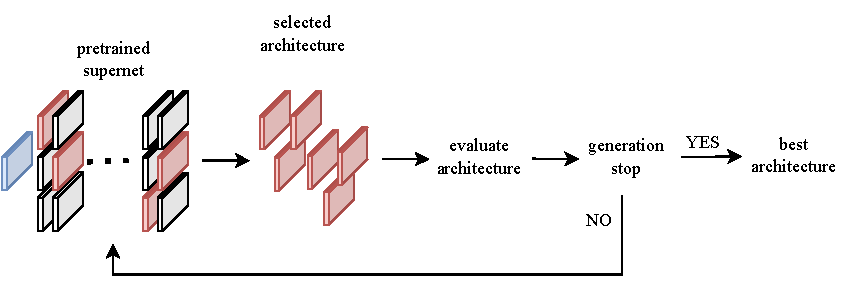
\includegraphics[width=\textwidth]{flow.pdf}
                \caption{
                    {\fontsize{12pt}{10pt}\selectfont
                        ASAGA的運作流程。
                        在每一世代中ASAGA會從訓練完成的超級網路隨機選擇架構進行評估,
                        並在最後一個世代結束時搜尋出表現最佳的模型架構。
                    }
                }
                \label{fig:ASAGA}
            \end{figure}

        \subsection{興趣指數}
            \label{subsec:point_of_interest}
            除了車流量和站點車輛數目,
            SAGAON也採用了鄰近站點的興趣指數作為輸入。
            我們使用Google API的地圖資訊,
            以站點為中心搜尋方圓200公尺內的興趣地點(interesting spot),
            利用笛卡爾座標系統(Cartesian coordinate system)將興趣地點的經緯度轉換成對應的座標,
            藉由興趣地點所構成的城市區域視為一個平行四邊形(parallelogram)並定義出2種構成該區域的向量,
            將對應的座標點放入劃分為同樣大小的$n \times n$的網格(grid)。
            我們將所有的興趣地點分為10類,
            分別為食物(food)、購物中心(mall)、商業(business)、醫院(hospital)、大眾傳輸(transportation)、政府組織(government)、公園(park)、公寓(apartment)、娛樂(entertainment)和運動(sport)。
            每個站點有10張不同種類的興趣點地圖(POI map),
            表示成$M_i \in \mathbb{R}_i^{10 \times n\times n}$,
            每張地圖代表特定的種類$a$。
            $\mu_{i,x}^a$為站點$i$、種類$a$在興趣點地圖座標$x$上的評價總數(rating amount)總和值。
            因應不同座標上評價總數值可能存在極大的差距,
            我們使用極值正規化(min-max normalization)來處理評價總數:
            \begin{equation}
                {\mu_{i,x}^a}' = \frac{\mu_{i,x}^a - \mu_{min}}{\mu_{max} - \mu_{min}} \in [0,1].
            \end{equation}
            評價總數經過正規化之後會和$\rho$進行運算,
            站點$i$、種類$a$在興趣點地圖座標$x$的興趣指數公式為:
            \begin{equation}
                M_{i,x}^a = \sum_{q=1}^{\gamma} ({\mu_{i,x}^{a,q}}' \times \rho_{i,x}^{a,q}).
            \end{equation}

        \subsection{最佳化模型超參數}
            超參數是深度學習一大重要設置,
            可大幅影響最終的訓練結果。
            然而我們無法事先得知與當前訓練資料最匹配的超參數組合,
            因此我們使用\xalg{alg:ASAGA}的變形,
            將搜尋的目標從神經網路架構調整為超參數組合,
            配合二進位編碼(binary encoding)來轉換各項不同的參數,
            方便於實作交配與突變運算子。
            \xfig{fig:crossover}、\xfig{fig:mutation}展示了交配運算子與突變運算子的實際流程,
            類基因演算法中兩者分別代表鄰近(lcoal)和全域(global)搜尋,
            嘗試在有限的資源條件下找出最佳的適應解。
            \begin{figure}[htb]
                \centering
                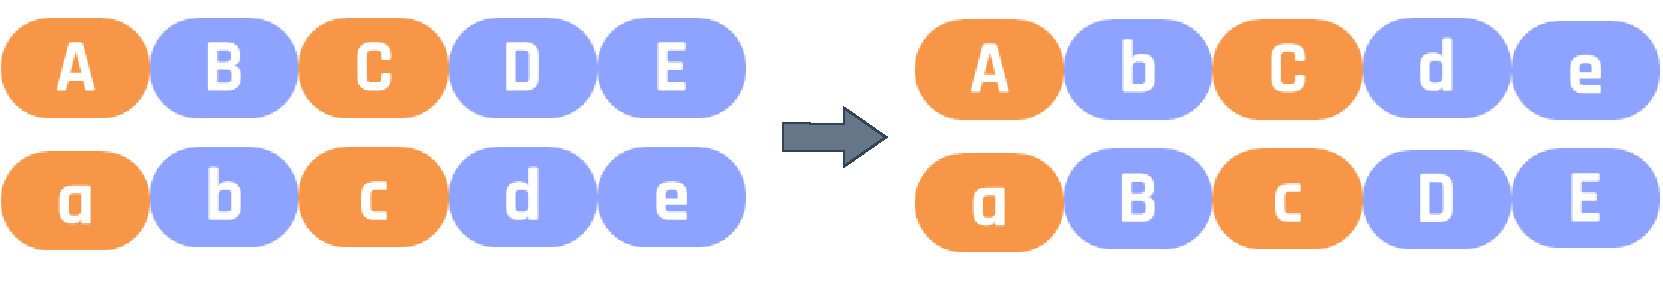
\includegraphics[width=\textwidth]{crossover.pdf}
                \caption{
                    {\fontsize{12pt}{10pt}\selectfont
                        交配運算子示例。
                        本專案使用多點(plural-points)交配運算,
                        在每次交配時隨機選出多個交配點(crossover point)來進行基因交換。
                        在此範例中被選定的交配點用藍色區塊來表示。
                    }
                }
                \label{fig:crossover}
            \end{figure}
            \begin{figure}[htb]
                \centering
                
\includegraphics[width=\textwidth]{mutation.pdf}
                \caption{
                    {\fontsize{12pt}{10pt}\selectfont
                        突變運算子示例。
                        此專案採用多點突變,
                        每次進行突變操作時隨機選出多個突變點進行布林(Boolean)反向運算。
                        在此範例中被選定的突變點用淺綠色來示意。
                    }
                }
                \label{fig:mutation}
            \end{figure}

            \xfig{fig:SAGA_scheme}是自適應模擬退火基因演算法作用於尋找最佳超參數的完整流程。
            在一開始該演算法會隨機產生一個新的群集以進行交配與突變的操作,
            並在評價後用得到的適應度進行模擬退火篩選(SA-selection),
            增加搜尋空間的彈性,
            避免落入區域最佳解之窠臼。

            \begin{figure}[!htb]
                \centering
                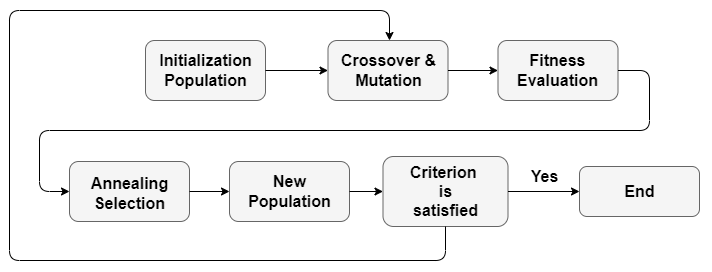
\includegraphics[width=0.725\textwidth]{SAGA_scheme.png}
                \caption{
                    {\fontsize{12pt}{10pt}\selectfont
                        自適應模擬退火基因演算法尋找最佳超參數的完整流程。
                    }
                }
                \label{fig:SAGA_scheme}
            \end{figure}
            

    \newpage

    \section{實驗}
        \subsection{環境設置}
            
            所有的實驗皆在Intel Core i5-8400 CPU (2.80GHz)、32 GB DDR4 RAM、NVIDIA RTX-2060 GPU with 6 GB VRAM的單一臺電腦上執行,
            作業系統為Windows 10,
            使用Python 3.8.13、Tensorflow-GPU 2.5.0和Keras 2.4.3來撰寫程式。
            資料集使用的是New York Citi Bike於2020年7月1日至2020年8月29日的公開資料,
            每筆紀錄皆含有開始/結束站點、借車/還車的時間。
            資料集被分為2個部分,
            2020年7月1日到2020年8月9日這40天被當作訓練用資料集,
            剩下的20天資料(2020年8月10日到2020年8月29日)則當作測試用。
            我們藉由總流量($\lvert$流入量$\rvert + \lvert$流出量$\rvert$)篩選出前100個流量最大的站點作為預測目標,
            關係密切的站點會被劃分到同一個群組,
            作為車流量特徵的計算依據。
            我們還添加了額外特徵如天氣和興趣指數來增加準確率。
            天氣資訊使用公開網站(\url{https://www.wunderground.com/})
            於2020年7月1日到2020年8月29日的觀測資料,
            每筆紀錄包含了紐約的溫度、降雨、濕度等資訊。
            我們使用極值正規化來處理這些特徵值並在預測後進行逆正規化(denormalize)。

        \subsection{神經網路架構搜尋前處理}

            \subsubsection{再平衡對於公共自行車系統的影響}
                \label{subsubsec:rebal}
                由於真實資料集中存在的雜訊和資訊缺失,
                前處理方法也會大幅影響預測的準確率。
                在實作New York Citi Bike資料集前處理時
                所遇到最大的困難便是站點車輛資料的缺失,
                紐約市政府並沒有公開各站點的歷史車輛數目,
                且在進行車輛再平衡(rebalancing)時並不會有操作紀錄,
                若是直接從租借紀錄還原車輛數目會存在落差,
                從而導致預測失準。
                為了解決這個問題,
                我們發現車輛紀錄的連貫性,
                若第$n$筆紀錄的結束站點與第$n + 1$筆紀錄的起始站點不相同,
                便能推測這台車輛有經過工作人員再平衡,
                我們也稱這種情況為幽靈騎者(ghost rider)。
                藉由借閱紀錄和再平衡的逆推,
                我們便能盡量還原真實的站點車輛數目。

            \subsubsection{車流量}
                \label{subsubsec:flow}
                就如\xsec{subsec:spatial_temporal}提到,
                與STDN所使用的前處理方式不同,
                我們認為使用地理位置建構車流量特徵並不足以精準體現站點間的關係,
                舉例來說,
                若有2個流量來往密切的站點距離過遠,
                使用地理位置劃分便有可能忽略這2個站點間的相互關係。
                以站點為基準的前處理方法就是為了解決這項問題而提出的發想,
                我們首先篩選出了100個總流量最大的站點並把它們稱為主要車流站點(major flow station),
                接下來針對每一個目標站點尋找出在特定時間區段內與其擁有密切流量的站點,
                彙整為該目標的站點群組。
                為了找出各站點對應的群組,
                我們觀察主要車流站點之間的車流量,
                並將超過最大流量50\%的站點歸類到預測目標的站點群組,
                最後以目標站點為中心,
                找出群組裡離該站點最遠的站點,
                以它為比例尺進行縮放,
                並利用笛卡爾座標系統進行轉換,
                定義出囊括了群組中所有站點的平行四邊形與2種構成該區域的向量,
                把所有站點的車流量特徵標註到$n \times n$的網格裡。

            \subsubsection{站點車輛數目}
                利用\xsec{subsubsec:rebal}的車流量特徵和再平衡方法,
                便能夠還原站點車輛數目特徵。
                我們將資料以每30分鐘進行劃分,
                利用站點間的流量,
                估算出在時間區段的起始和結束當下目標站點中的自行車數量。
                如先前所說,
                由於沒有實際的站點車輛數,
                上述流程推估出來的為相對的車輛浮動值。
                為避免在逆推時造成腳踏車數量負值,
                我們會對預測值進行檢查,
                若為負值則會進行平移以確保預測值合理。

            \subsubsection{參數設定}
                \label{subsubsec:parameters_setting}
                在我們的實驗中,批次大小(batch size)設定為64,
                學習率(learning rate)則是0.001。
                訓練尋獲的神經網路模型使用了提前停止機制(early stop),
                用以縮短訓練時間。
                我們設定自適應模擬退火基因演算法的世代(generation)數目為10、族群則為20。
                初始的溫度為1,
                搭配上0.9的冷卻率。
                在評價結果時我們會過濾掉站點車輛數目值時小於15的部分。

            \subsection{超參數優化前處理}
                \subsubsection{編碼設計}

                    在STDN之中共有5種使用者可自行更動之參數,
                    分別為注意力長短期記憶模型數量(att\_lstm\_num)、長效型長短期記憶模型數量(long\_term\_lstm\_num)、短效型長短期記憶模型數量(short\_term\_lstm\_num)、鄰近區域大小(nbhd\_size)與卷積神經網路鄰近區域大小(cnn\_nbhd\_size)。
                    這些可調整之參數都是十進位的整數,
                    為使其能夠進行交配和突變此類基因演算法所需操作,
                    我們對這些參數採用二進位的編碼方式。
                    \xfig{fig:chromosome_sheme}是由STDN超參數所構成的染色體示意圖。
                    \begin{figure}[htbp]
                        \centering
                        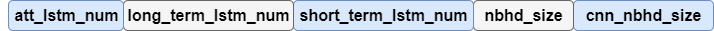
\includegraphics[width=\textwidth]{chromosome_sheme.png}
                        \caption{
                            {\fontsize{12pt}{10pt}\selectfont
                                STDN參數轉換成適用於該框架之染色體之預覽圖。
                            }
                        }
                        \label{fig:chromosome_sheme}
                    \end{figure}

                \subsubsection{參數設定}

                    我們設定自適應模擬退火基因演算法的世代數目為5、族群大小則為6。
                    交配與突變的機率分別為0.8與0.2。
                    初始的溫度為1.5,
                    搭配上0.8的冷卻率(cooling ratio)。
                    每個區塊的長度根據事前規定的參數範圍來變動,
                    \xtab{tab:range}為該專案中在所有超參數的範圍規定。
                    由於STDN的原始設計,
                    注意力長短期記憶模型數量、長效型長短期記憶模型數量和短效型長短期記憶模型數量的數值必須大於1,
                    且長效型長短期記憶模型數量必須為奇數。
                    我們使用事先定義好的上下限來組成左閉右開的半開區間(half-open interval)。
                    參數的上限值依實驗設備可進行適量地調升,
                    然而大部分深度學習模型訓練所需時間與資源與參數大小呈正相關,
                    為證明該策略有效性,
                    我們期待能夠以一組數值更小的超參數來獲得同等於或優於原論文的成果,
                    因此在此實驗中各項超參數的上限即為原論文所使用的預設參數。

                    \begin{table}[htbp]
                        \caption{
                            {\fontsize{12pt}{10pt}\selectfont
                                超參數範圍
                            }
                        }
                        \centering
                        \begin{NiceTabular}{|c|c|c|}
                            \CodeBefore
                                \rowcolor[HTML]{C0C0C0}{1}
                                \rowlistcolors{2}{white, gray!25}[restart]
                            \Body
                                \hline
                                \textbf{參數名稱} & \textbf{下限} & \textbf{上限} \\
                                \hline
                                注意力長短期記憶模型數量 & 2 & 4 \\
                                \hline
                                長效型長短期記憶模型數量 & 3 & 8 \\
                                \hline
                                短效型長短期記憶模型數量 & 2 & 8 \\
                                \hline
                                鄰近區域大小 & 0 & 4 \\
                                \hline
                                卷積神經網路鄰近區域大小 & 0 & 4 \\
                                \hline
                        \end{NiceTabular}
                        \label{tab:range}    
                    \end{table}

        \subsection{實驗結果}
            
            \subsubsection{神經網路架構搜尋成果}

                \xtab{tab:comparison}和\xfig{fig:comparison}展示了SAGAON對比其他基線實驗(baseline)在紐約市公共自行車資料集的預測結果,
                每種方法都執行了5次並紀錄平均值和標準差。
                SAGAON勝過了所有的基線實驗,
                均方根誤差跟平均絕對百分比誤差(mean absolute percentage error ; MAPE)在測試資料集上皆為最低。
                \begin{table}[htb]
                    \caption{
                        {\fontsize{12pt}{10pt}\selectfont
                            基線實驗和SAGAON之間的比較
                        }
                    }
                    \centering
                    \newcommand{\z}{\phantom{0}}
                    \resizebox{\columnwidth}{!}{
                        \begin{NiceTabular}{|c|r|r|r|r|}
                            \CodeBefore
                                \rowcolor{lightgray}{8}
                            \Body
                                \hline
                                &\multicolumn{2}{c}{Start}& \multicolumn{2}{c}{End}\\[2pt]
                                \hline
                                Method &  \multicolumn{1}{c}{RMSE$\ \downarrow$} &  \multicolumn{1}{c}{MAPE$\ \downarrow$} & \multicolumn{1}{c}{RMSE$\ \downarrow$}& \multicolumn{1}{c}{MAPE$\ \downarrow$}  \\
                                \hline
                                ARIMA & 11.43$\pm$0.00 & 73.89$\pm$0.00 & 11.78$\pm$0.00 & 75.99$\pm$0.00 \\ 
                                HA & \z8.56$\pm$0.00 & 67.24$\pm$0.00 & 8.57$\pm$0.00 & 67.51$\pm$0.00 \\ 
                                LSTM & \z2.97$\pm$0.73 & 17.66$\pm$0.29 & 4.13$\pm$0.12 & 25.59$\pm$0.74\\
                                Conv-LSTM & \z2.13$\pm$0.31 & 11.11$\pm$1.23 & 3.36$\pm$0.26 & 19.88$\pm$0.44 \\
                                STDN & \z2.07$\pm$0.23 & 10.83$\pm$0.80 & 3.33$\pm$0.16 & 20.23$\pm$0.90 \\
                                \hline
                                \textbf{SAGAON} & \textbf{2.07$\pm$0.03} & \textbf{10.81$\pm$0.12} & \textbf{3.31$\pm$0.06} & \textbf{19.10$\pm$0.17} \\
                                \hline
                        \end{NiceTabular}}
                    \label{tab:comparison}    
                \end{table}
                
                HA和ARIMA這類的傳統時序預測方法相當不準確,
                因為它們只依靠過去的歷史紀錄來預測,
                忽略了空間特徵。
                SAGAON也勝過了長短期記憶模型、卷積長短期記憶模型和STDN這類深度學習方法,
                潛在原因可能是SAGAON對於空間與時間特徵的處理更為妥當。
                長短期記憶模型只關心過去連續的時序資料,
                忽略了空間資料;
                卷積長短期記憶模型使用卷積層來捕捉空間特徵,
                並保留了長短期記憶模型的優勢。
                STDN使用空間-時間相混的資料來進行訓練,
                用以捕捉了動態空間相似性(dynamic spatial similarity)和週期時間遞移性(periodic temporal shifting),
                這也是它的結果能夠勝過其他模型的決定性因素。
                以STDN為基礎,
                我們提出的SAGAON增添了one-shot NAS的超級網路,
                藉由選擇不同的選擇模塊來增加訓練的準確率,
                同時因為透過超啟發式演算法ASAGA作為搜尋策略,
                SAGAON在搜尋架構的過程中可以減少許多時間和計算資源。

                \begin{figure}[htb]
                    \centering
                    \begin{subfigure}{.5\columnwidth}
                        \centering
                        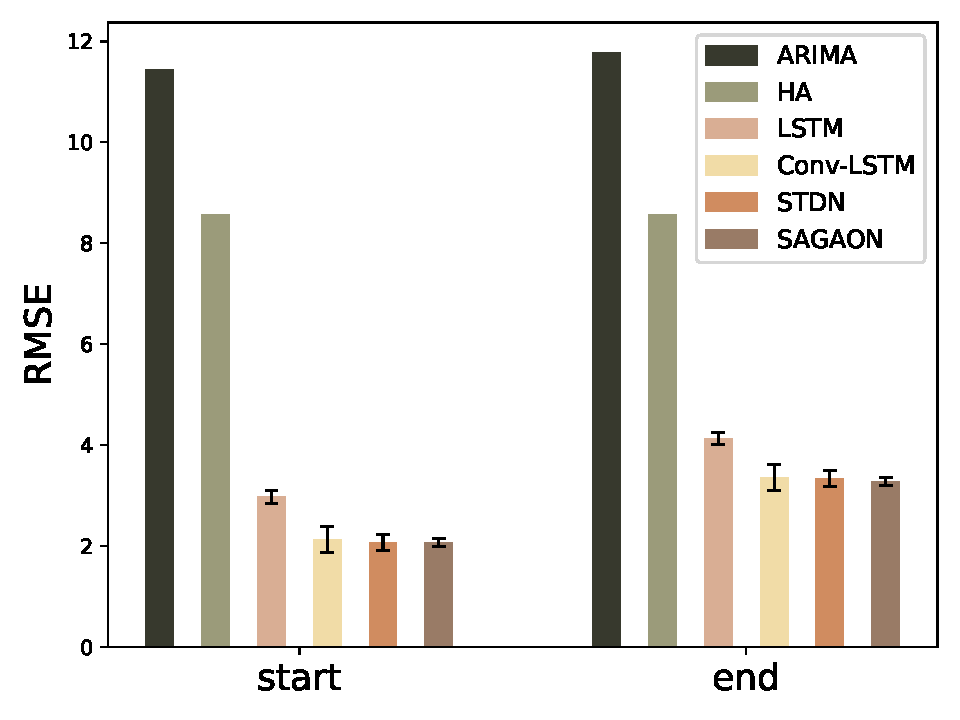
\includegraphics[width=\linewidth]{station_level_RMSE.pdf}
                        \caption{
                            {\fontsize{12pt}{10pt}\selectfont
                                Station-level RMSE
                            }
                        }
                    \end{subfigure}%
                    \hfill
                    \begin{subfigure}{.5\columnwidth}
                        \centering
                        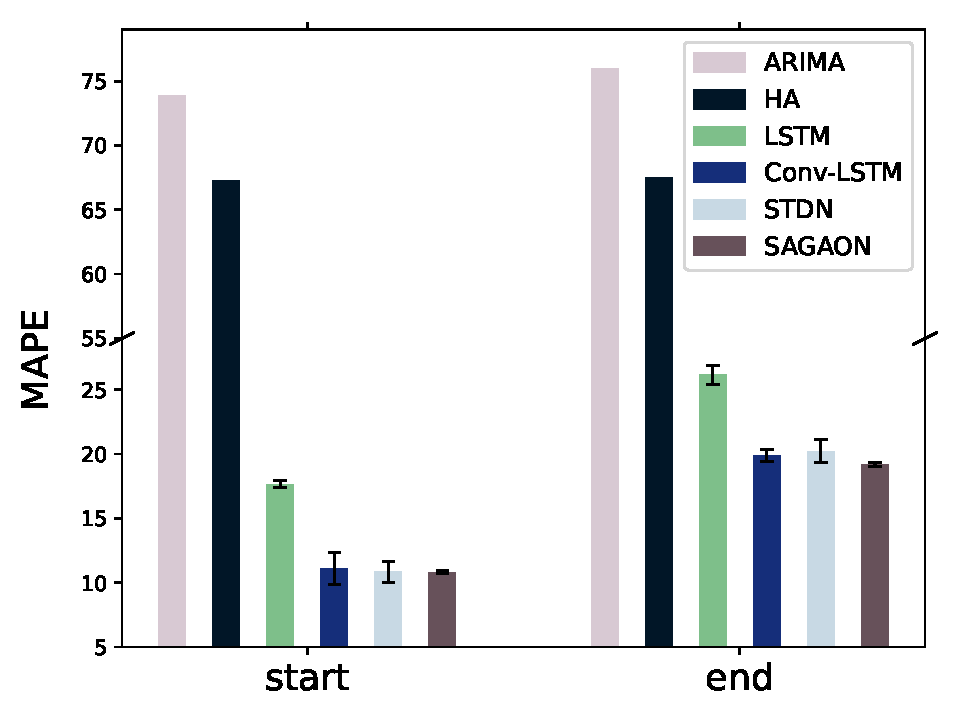
\includegraphics[width=\linewidth]{station_level_MAPE.pdf}
                        \caption{
                            {\fontsize{12pt}{10pt}\selectfont    
                                Station-level MAPE
                            }
                        }
                    \end{subfigure}%
                    \caption{
                        {\fontsize{12pt}{10pt}\selectfont
                            SAGAON對比不同的基線實驗模型
                        }
                    }
                    \label{fig:comparison}
                \end{figure}

            \subsubsection{超參數優化成果}
                \xtab{tab:hyper_comparison}是論文預設實驗與套用了超啟發演算法參數搜尋策略的對比。
                每種方法都執行了3次並紀錄平均值和標準差。
                傳統的基因演算法及我們提出了自適應模擬退火基因演算法皆得到比預設參數更好的實驗結果。
                SAGA在預測租借車輛的部分擁有較亮眼的表現,
                GA則是在歸還車輛的部分有突出的效果。
                SAGA與GA所選定的超參數序列皆小於預設參數,
                證明了在超啟發演算法的幫助下我們能夠以更少的運算資源取得更好的表現。
                此優化得益於超啟發演算法的泛用性,
                無需使用者先行理解該框架的背景知識即可運用。
                \begin{table}[htbp]
                    \caption{
                        {\fontsize{12pt}{10pt}\selectfont
                            預設參數和採用了超啟發演算法搜尋策略之間的比較
                        }
                    }
                    \begin{NiceTabular}{|c|r|r|r|r|}
                        \CodeBefore
                            \rowcolor{lightgray}{5}
                        \Body
                            \hline
                            & \multicolumn{2}{c}{Start} & \multicolumn{2}{c}{End} \\[2pt]
                            \hline
                            Method & \multicolumn{1}{c}{RMSE$\ \downarrow$} &  \multicolumn{1}{c}{MAPE$\ \downarrow$} & \multicolumn{1}{c}{RMSE$\ \downarrow$}& \multicolumn{1}{c}{MAPE$\ \downarrow$}  \\
                            \hline
                            Default & 8.85$\pm$0.11 & 21.84$\pm$0.36 & 8.15$\pm$0.15 & 20.87$\pm$0.39 \\ 
                            Genetic Algorithm & 8.83$\pm$0.06 & 21.60$\pm$0.21 & 8.14$\pm$0.03 & 20.42$\pm$0.18 \\ 
                            \hline
                            \makecell[c]{\textbf{Simulated Annealing} \\ \textbf{Genetic Algorithm}} & \textbf{8.81$\pm$0.04} & \textbf{21.63$\pm$0.16} & \textbf{8.15$\pm$0.07} & \textbf{20.66$\pm$0.04} \\
                            \hline
                    \end{NiceTabular}
                    \label{tab:hyper_comparison}    
                \end{table}

        \subsection{使用者介面設計}
            為了視覺化實驗結果以利快速掌握系統各站點現況,
            我們架設了一個簡單的網站來呈現模型在每個不同時間區間對每個站點預測的結果,
            並且以顏色來區分預測結果之好壞。
            我們運用開源的框架及模組來架構網頁基礎,
            搭配應用程式介面(application programming interface ; API)來快速構建出所需的視覺呈現效果。
            我們使用了以下的開源工具來完成這項工作:
            \begin{itemize}
                \item 框架 → Django: \\
                    Django是一個以Python所建立的模組模板可視化(model-template views ; MTV)網路框架。
                \item 非同步請求(asynchronous request) → Asynchronous JavaScript and XML (Ajax): \\
                    Ajax是一個能讓網站能在不用刷新頁面的情況下自動從資料庫抓取資料的一個請求方法(request method)。
                \item Javascript第三方程式庫 → chart.js: \\
                    我們引用了chart.js這個函式庫輔助網頁上視覺化作圖的部分。
                \item 資料庫 → MySQL: \\
                    我們建立了一個專用的MySQL資料庫用以存各站點的所有腳踏車數量,
                    包含了真實數量(ground truth)及模型預測數量(predict value)。
                \item 應用程式介面 → Google Maps JavaScript API: \\
                    Google Maps JavaScript API用來呈現美國紐約市的地圖,
                    並以客製化標記(custom marker)來代表各個目標站點。
            \end{itemize}

            \xfig{fig:webpage}是成果頁面的整體架構。
            前後端的部分皆是使用Django預設的網路框架。
            在原先計畫中有考慮使用React或是Angular等更細緻化的前端框架,
            但考慮到時間成本因此最後並沒有採用。
            \begin{figure}[htb]
                \centering
                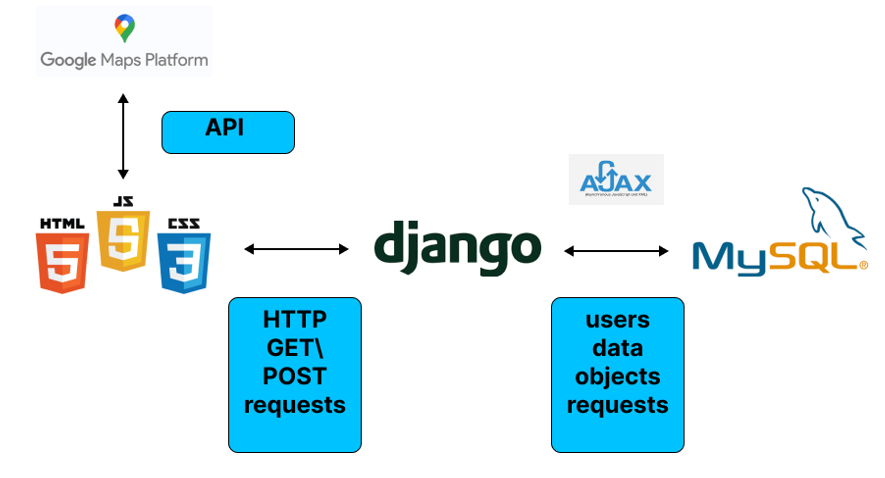
\includegraphics[width=0.8\textwidth]{webpage.png}
                \caption{
                    {\fontsize{12pt}{10pt}\selectfont
                        網頁整體框架。
                    }
                }
                \label{fig:webpage}
            \end{figure}

            為了負荷後端系統龐大資料量的輸入輸出,
            我們採用了非同步系統的架構。
            非同步讓我們可以在不主動更新頁面的情況下,
            利用Ajax來更新網頁內容。
            舉例來說,
            Instagram與Facebook等大型社交媒體能夠在不重新整理頁面的前提下獲得新的內容,
            這就是Ajax的基本應用。
            \xfig{fig:asynchronous}簡單示意了同步與非同步請求的差別。
            可以看到傳統的同步請求必須在一次請求之後必須馬上回覆一次,
            這在處理大量資料時會造成等待時間過久,
            非同步請求則能有效解決掉這方面的困擾。
            \begin{figure}[htbp]
                \centering
                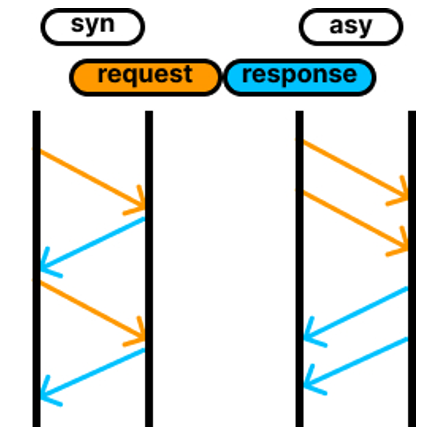
\includegraphics[width=0.35\textwidth]{asynchronous.png}
                \caption{
                    {\fontsize{12pt}{10pt}\selectfont
                        同步請求與非同步請求的差別。
                    }
                }
                \label{fig:asynchronous}
            \end{figure}

            \xfig{fig:web-view}是網頁的主要介面,右側面板為當前天氣狀況,左側則是100個目標站點在
            當前時間點的模型預測狀況以及真實站點車輛數。每次更新的時間為15分鐘一次,為快速呈現模型成果,
            我們每三秒即更新一次介面。
            \begin{figure}[htb]
                \centering
                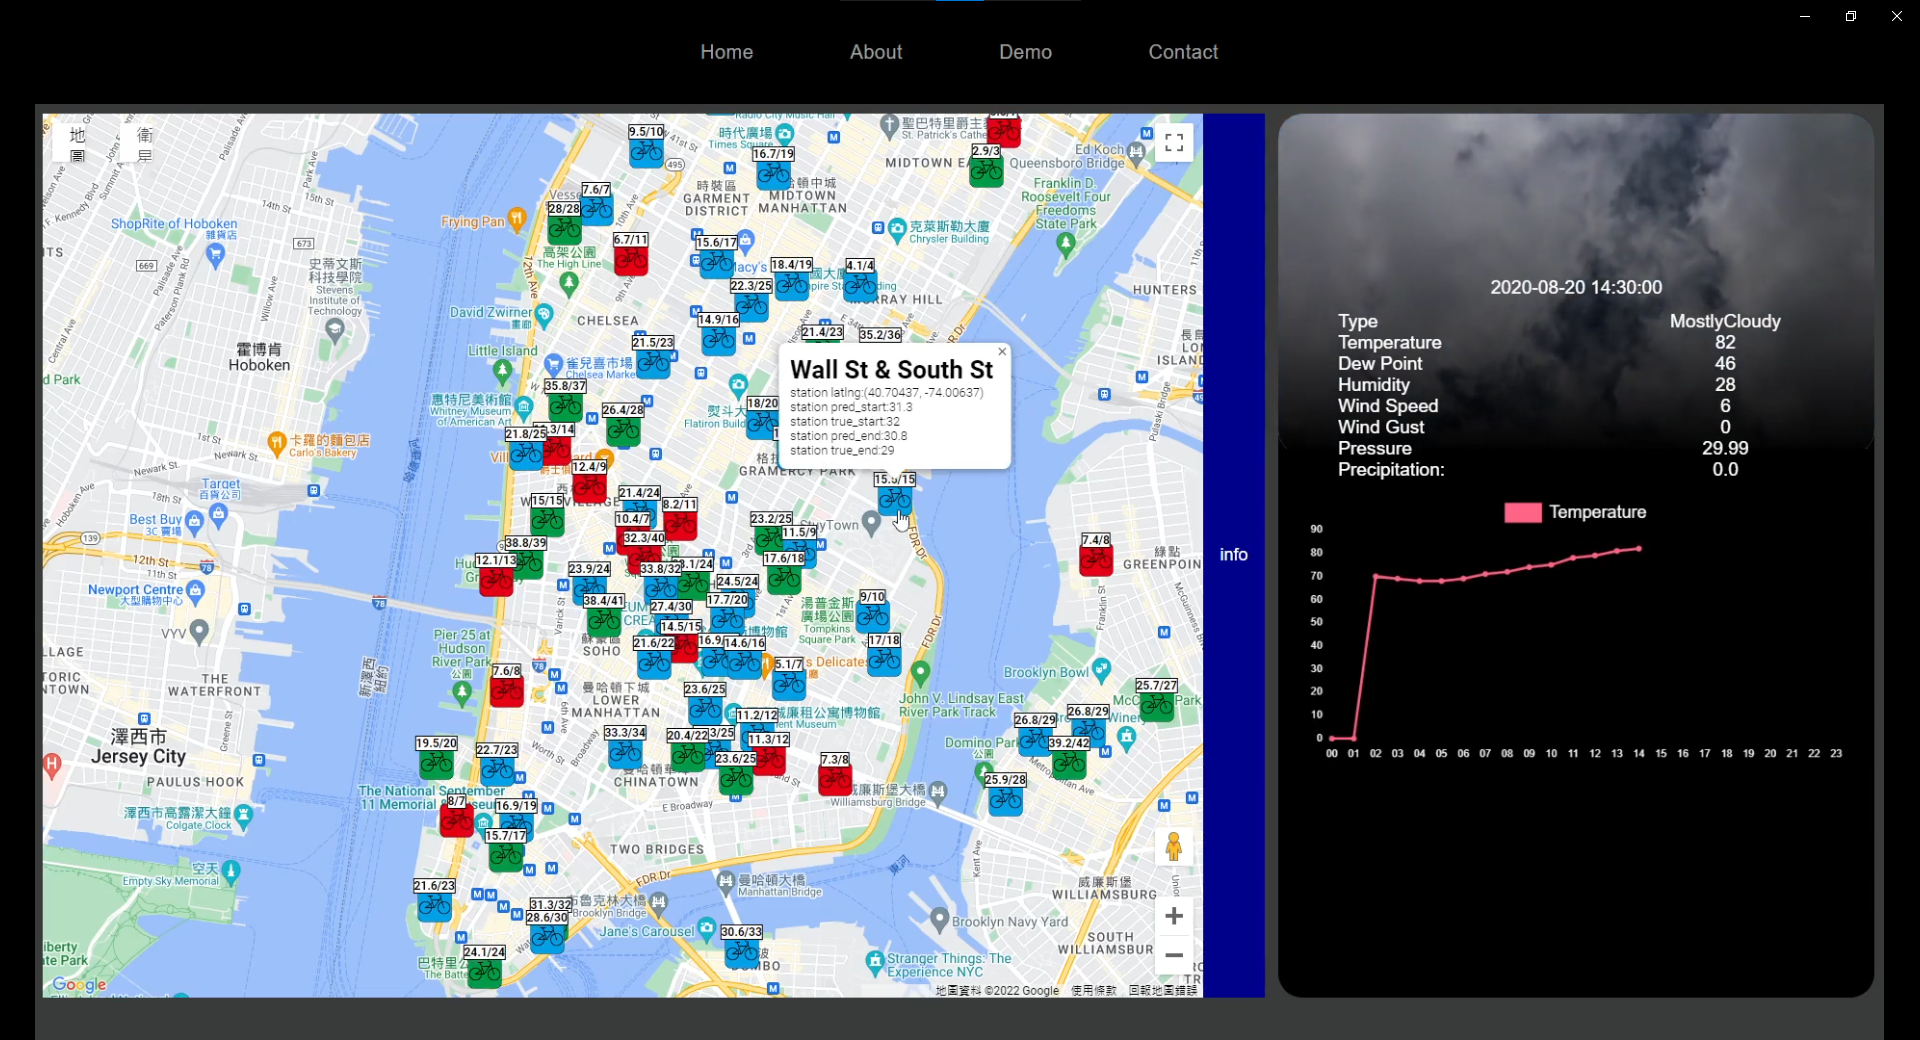
\includegraphics[width=\textwidth]{nstc_adjust_image.png}
                \caption{
                    {\fontsize{12pt}{10pt}\selectfont
                        紐約市站點需求預測地圖。
                    }
                }
                \label{fig:web-view}
            \end{figure}
            從使用者介面上可以看到三種顏色的區分,
            綠色代表相當準確,藍色為尚可接受,紅色則是預測結果和實際數值有落差,
            判斷站點不準確度的公式如下 \ref{acc_equ}。
            $S_p$是在此時間區間開始時模型預測的站點車輛數,
            $E_p$是時間區間結束時的預測結果。
            $S_t$和$E_t$則分別代表在此時間區間開始及結束的真實站點車輛數。
            如果不準確度達於0.2則站點及呈現紅色,
            小於0.06則呈現綠色,
            其餘裝快接為可接受範圍,
            呈現藍色。
            \begin{equation}
            \label{acc_equ}
            \text{$inaccuracy$} = \frac{|S_p-S_t|+|E_p-E_t|}{S_t+E_t}.
            \end{equation}

            \[
            colors =
            \begin{cases}
            red & \text{if $inaccuracy>0.2$} \\
            green & \text{if $inaccuracy<0.06$} \\
            blue & \text{else} 
            \end{cases}
            \]

            \xfig{fig:details}中間的面板呈現了當日預測狀況的折線圖,從折線圖每日的走向可以發現,當到尖峰時刻
            尤其是傍晚下班時,模型的預測準確度下降了許多,原因是因為隨著用量突然增加,模型在預測上也會有相對更高的誤差
            。我們也將不準確次數前10多的站點挑出來,以利日後可以針對站點來了解主要造成原因為何,以及我們可以如何改善。
            \begin{figure}[htbp]
                \centering
                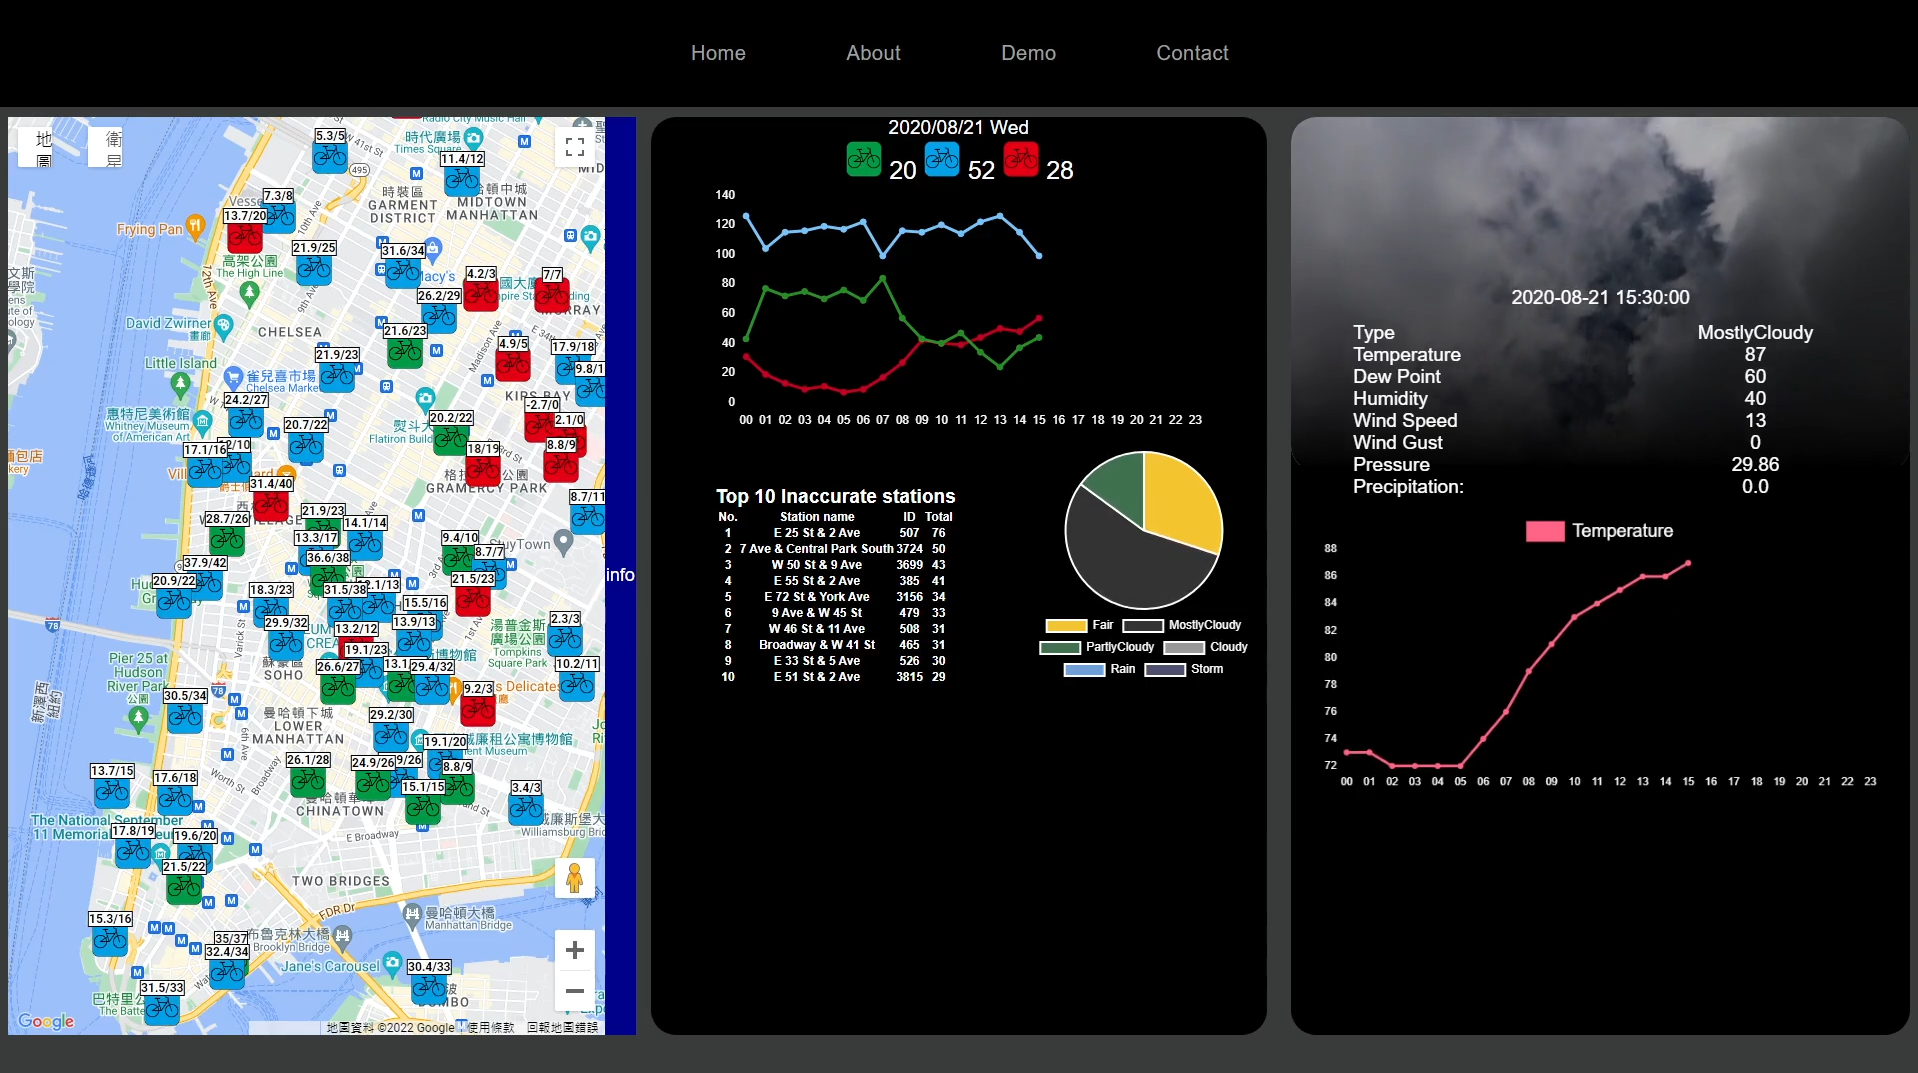
\includegraphics[width=\textwidth]{details.png}
                \caption{
                    {\fontsize{12pt}{10pt}\selectfont
                        當日預測情況以及每月預測最不準的站點。
                    }
                }
                \label{fig:details}
            \end{figure}

    \newpage
    \section{結論}
        
        在這項專題研究中,
        我們提出了模擬退火基因演算法one‑shot神經網路搜尋(SAGAON),
        一個針對公共自行車系統站點車流進行預測的神經網路搜尋框架。
        此框架藉由自動找尋出擁有高準確率的模型架構,
        改善了空間-時間相依性高的深度學習模型對於真實世界交通流問題的預測能力。
        根據資料集的測試,
        SAGAON即使與其它最先進的方法相比依然有相當高的競爭力。
        目前所使用的訓練資料為紐約市Citi Bike的歷史紀錄,
        我們在未來打算將該框架實際應用於高雄市的YouBike系統,
        嘗試將此系統與使用者介面應用在台灣YouBike2.0,
        這個使用者介面不僅能讓嘗試解決調度問題的系統開發人員有一個工具來了解各個時段、區域、天氣條件下各站點之狀況,
        也可以讓幕後人員能更快掌握整個系統當前情況。
        幫助相關的民間業者和政府組織改善公共自行車系統的使用狀況和效率。
        再者,
        我們將致力於改善該框架的訓練成本如訓練所需的計算資源與時間,
        如此一來便能讓SAGAON在更多資源有限的終端上運行。

    \newpage
    \section{未來工作與相關回饋}
        \subsection{未來工作}
            因為本專題實驗的硬體條件無法負荷更大量的數據,
            希望未來可以將資料量增加並使用更高效的硬體設備,
            我們相信這對模型預測的準確度會有幫助。另外因實驗所採用的是歷史資料,
            並沒有及時的資料可以應用,未來會希望能利用即時資料讓我們的模型可以在
            實際場景中應用。關於使用者介面的調整,我們將新增更多資料分析在主要預
            測面板上,除了即時的站點預測外,也希望能新增調度路線規劃給調度人員參考。
        \subsection{相關回饋}
            \begin{itemize}
                \item [\textbf{Q:}]
                是否有針對不同特徵值的處理及實驗結果?
                哪一些特徵值對結果的影響比較重要?
                \item [\textbf{A:}]
                在經過有無興趣指數和天氣特徵的實驗後,
                發現興趣指數對於準確度的影響較天氣明顯,
                不過某些條件下加入外部特徵會造成負面影響。
                \item [\textbf{Q:}]
                論文中提到該方法可以減少搜尋所需的時間與計算資源,
                在這方面是否有相關的論述與證明?
                \item [\textbf{A:}]
                經過測試220組不同模型架構的估算與實驗後,
                不使用one-shot方法的搜尋時間約為146小時,
                SAGAON大概為17小時,
                由此說明SAGAON可以在更少的時間內完成相同複雜的搜尋流程。
                \item [\textbf{Q:}]
                可以詳述如何把站點座標轉換成網格座標的嗎?
                \item [\textbf{A:}]
                在\xsec{subsec:point_of_interest}與\xsec{subsubsec:flow}提到了如何把興趣地點與目標站點的經緯度轉換成對應的網格座標。
                使用平行四邊形勾畫目標區域並找出2種構成該區域的對應向量,
                劃分出需要的網格大小以此完成座標化。
                \item [\textbf{Q:}]
                為什麼你們的模型是先壓縮空間特徵而不是時間特徵?
                請問這樣做的用意在於?
                \item [\textbf{A:}]
                使用CNN能夠優先過濾出重要的空間特徵,
                再把這些經過篩濾的資料送入LSTM進行時間相關的預測,
                通常這樣做的效果會比較好。
                未來可以嘗試改變模型來比較兩者不同之處。
            \end{itemize}

    \newpage
    \section{致謝和聲明}
        
        這項研究受到中華民國國家科學及技術委員會的協助,
        計畫編號NSTC 111-2813-C-110-033-E和NSTC 111-2222-E-110-006-MY3。
        關於前處理和模型的詳細程式碼,
        我們分別在(\url{https://github.com/YunYe0121/CitiBike_preprocessing})和(\url{https://github.com/B083040012/SAGAON})有更詳盡的說明。
        該專案之研究結果已整理齊全並已被IEEE Applied Sensing Conference\cite{SAGAON}所接受,
        已於2023年1月在該研討會口頭發表。

    \clearpage
    \stepcounter{section}
    \phantomsection
        \addcontentsline{toc}{section}{\texorpdfstring{\arabic{section}\hspace{1em}參考文獻}{參考文獻}}
        \renewcommand\refname{\arabic{section}\hspace{1em}參考文獻}
        \bibliographystyle{IEEEtran}
        \bibliography{nstc_report}

\end{document}
